\chapter{Arquitetura proposta}

\section{Visão geral do sistema}

\begin{figure}[H]
  \centering
  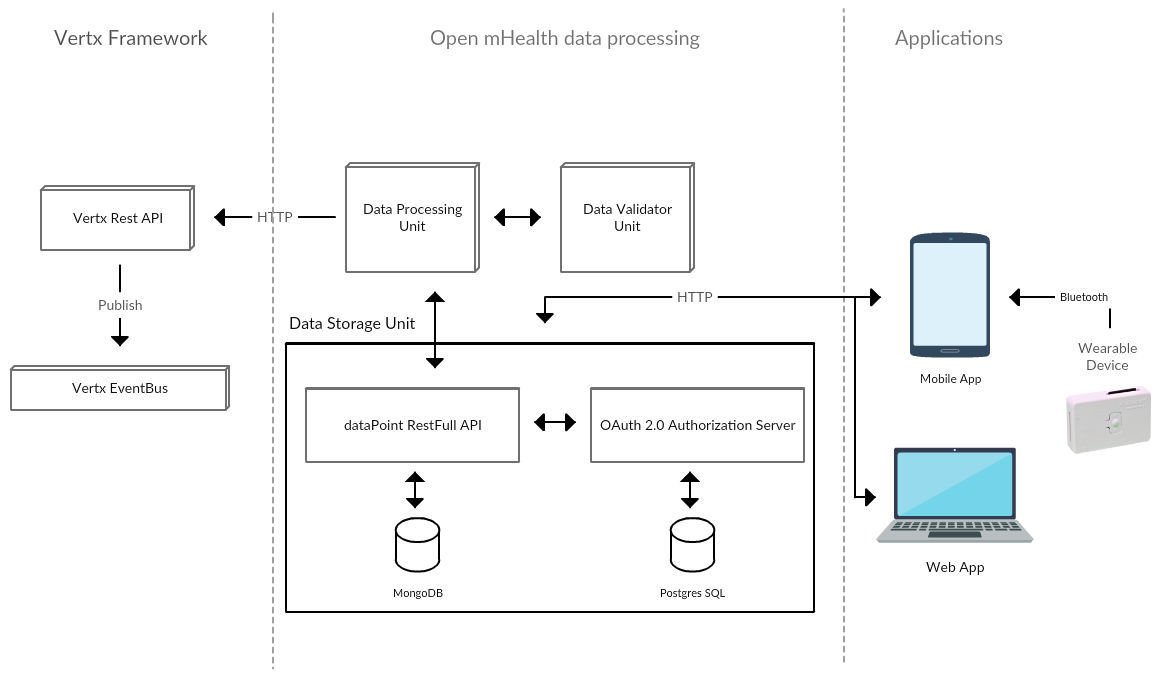
\includegraphics[width=1\textwidth]{imgs/arch-product.png}
  \caption[Arquitetura proposta para o Sistema]{Arquitetura proposta para o Sistema}
  
  \label{f:product-arch}
\end{figure}

A arquitetura proposta para o sistema está dividida em três partes. Uma delas é a parte das aplicações desenvolvidas, ou seja, a interface com o utilizador, tanto web como móvel. Estas duas aplicações comunicarão por pedidos \gls{HTTP} com o \gls{DSU} da framework do Open mHealth. A aplicação móvel ainda terá a responsabilidade de recolher os dados fisiológicos dos participantes como por exemplo o \gls{ECG}, a frequência cardíaca e o acelerómetro. O sensor utilizado para recolher os dados foi o VitalJacket \footnote{http://www.sdk.vitaljacket.com/?pageid=13} utilizando o perfil de bluetooth \gls{SPP}.
\par 
Uma outra parte do sistema já referida é o backend do Open mHealth. Este backend tem um componente principal (\gls{DSU}) que disponibilizará duas \gls{REST} \gls{API} para inserção e fornecimento dos dados e ainda para autenticação e autorização. Ainda terá um componente para processar os dados recebidos. Estes dados passarão por um validador e podem ser reencaminhados para uma framework para posterior publicação das mensagens num ''EventBus''.
\par
A terceira e última parte será composta uma framework que irá disponibilizar um ''endpoint'' para receber os dados e então publicar os mesmos no ''EventBus''.







\section{Módulos do sistema}
\subsection{Fundações do backend}
Para o backend do sistema será utilizado o Open mHealth adaptando-o no necessário e complementado-o. O backend deverá ser capaz de fornecer um serviço de autenticação e autorização seguindo o protocolo OAuth 2.0. \par 
Deverá disponibilizar uma \gls{API} para ser efetuado a inserção de dados fisiológicos dos utilizadores. Esta inserção será apoiada por um validador que irá validar esses dados, para perceber se podem ser aceites com sucesso.


\subsection{Extensão para suportar pipelines de processamento}
O backend do \gls{OMH} não suporta uma pipeline de processamento dos dados, para este suporte ser possível incluímos uma forma de os dados serem enviados para módulos interessados no seu processamento. A solução proposta passa pela publicação destes dados num event bus, permitindo a extensibilidade do sistema com facilidade e um tratamento especifico por cada um desses módulos.


\subsection{Integração das Aplicações}
As aplicações que forem desenvolvidas utilizando esta arquitetura proposta poderão utilizar, o servidor de autenticação e autorização fornecido pelo backend e também uma \gls{API} para efetuar a inserção e a consulta dos dados inseridos. Esta \gls{API} terá ainda a capacidade de validar os dados recebidos, e uma nova consulta de dados na perspetiva do Revisor. O conjunto de dados será mais extenso, pois serão adicionados mais esquemas de dados(\gls{ECG}, dados demográficos e acelerómetro) e a possibilidade de adicionar um novo módulo para processamento de novos dados recebidos do seu interesse.





\section{Modelo do domínio}
Será necessário guardar dados demográficos do utilizador e os dados fisiológicos como dados do acelerómetro, frequência cardíaca e \gls{ECG}. Para isso vou de seguida mostrar um diagrama de classes que podia ser a solução para o desenvolvimento de uma base de dados, tendo em conta os dados que precisamos de guardar.

\begin{figure}[H]
  \centering
  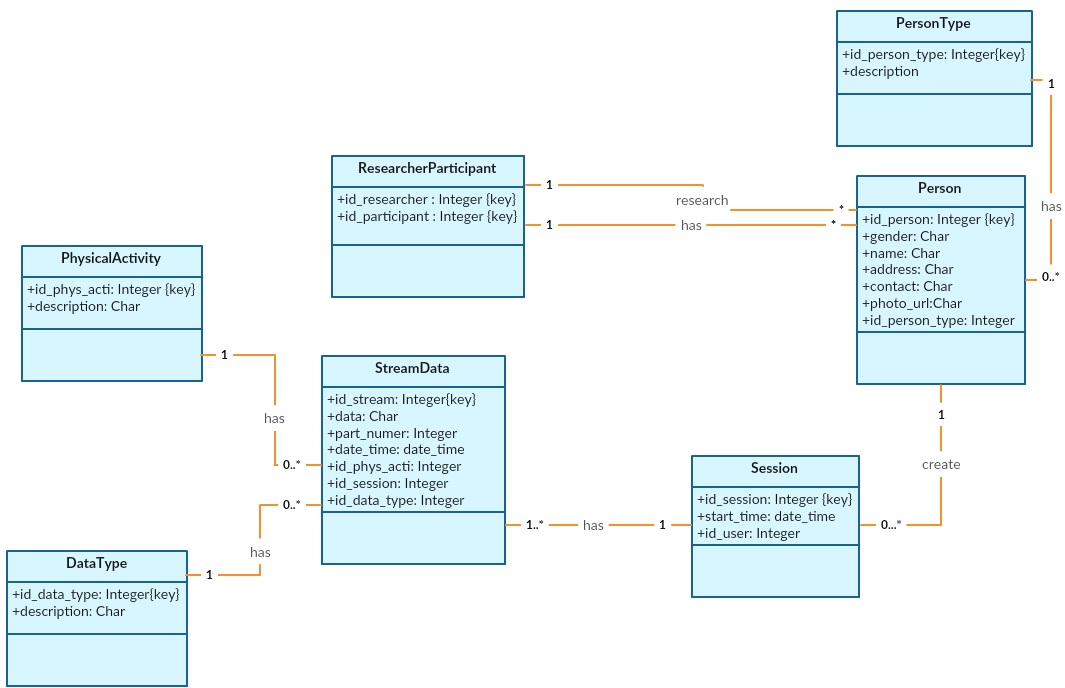
\includegraphics[width=1\textwidth]{imgs/class-diagram.png}
  \caption[Diagrama de classes para a arquitetura proposta]{Diagrama de classes para a arquitetura proposta}
  
  \label{f:class-diagram}
\end{figure}

Com este diagrama conseguimos guardar a criação de novas pessoas, que podem ser um utilizador normal ou um investigador/revisor. Conseguimos adicionar utilizadores a Revisores, e criar sessões relacionadas com um determinado utilizador definido a hora de inicio. Podem ser associadas a estas sessões novas leituras diferentes que irão ter um tipo de leituras associado e uma atividade física atual.
\par 
Existe ainda a possibilidade de utilizar uma base de dados não relacional, como por exemplo, orientada a documentos. Este tipo de bases de dados não depende de um esquema em especifico e como tal suporta dados não estruturados. Este modelo tem uma grande simplicidade permitindo assim aos utilizadores compreender facilmente o documento e aos programadores  obter os documentos sob a forma de arrays associativos \cite{nosql}. Uma das grandes vantagens que pode haver ao utilizar um base de dados orientada a documentos, é que a adição de novos esquemas de dados não vai implicar alterações ao esquema da base de dados, mesmo que os dados inseridos não estejam relacionados com os já existentes.





\section{Proteção de dados}
\label{cap6:protecaodados}
Relativamente à privacidade e aos dados armazenados, pode ser visto como uma questão de controlo de acesso, em que é assegurado que os dados estarão acessíveis apenas para pessoas e processos autorizados. Os serviços \gls{REST} deverão verificar se o pedido efetuado é ou não autorizado, para isso o utilizador deverá efetuar a autenticação e utilizar o token de acesso fornecido. O backend deverá utilizar duas bases de dados diferentes, em que numa delas guarda os dados relativos às aplicações cliente e os tokens de acesso, e na outra deverá guardar os dados inseridos e os dados relacionados com as contas de utilizador, protegendo assim dados fisiológicos e sensíveis dos utilizadores, da base de dados onde estão os tokens, deste modo conseguimos ter uma segregação de responsabilidade.

\cleardoublepage